\subsection{Kinematic Model Calculation}
\begin{comment}
    \begin{figure}[h]
        \centering
        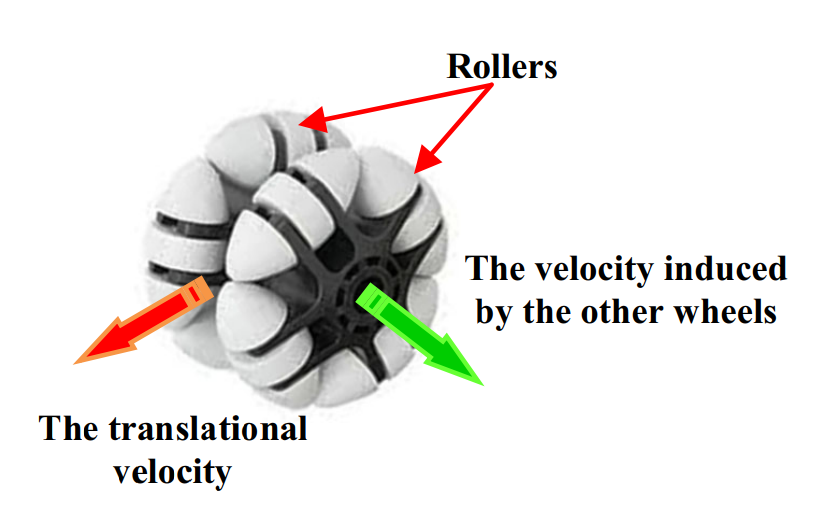
\includegraphics
            [width=0.4\textwidth]
            {figures/omniwheel.png}
        \caption{I}
        \label{fig:omniwheel}
    \end{figure}
    \end{comment}
    
    
\subsubsection{Induced velocity}
Assuming that only the wheel 3 rotates with a velocity $\dot{q_{3}}$ and the other two wheels are inactive we can define as induced velocity the velocity that wheels 1 and 2 gains from wheel 3. This velocity is perpendicular to the normal direction of rolling. This velocity is calculated from the next figure:

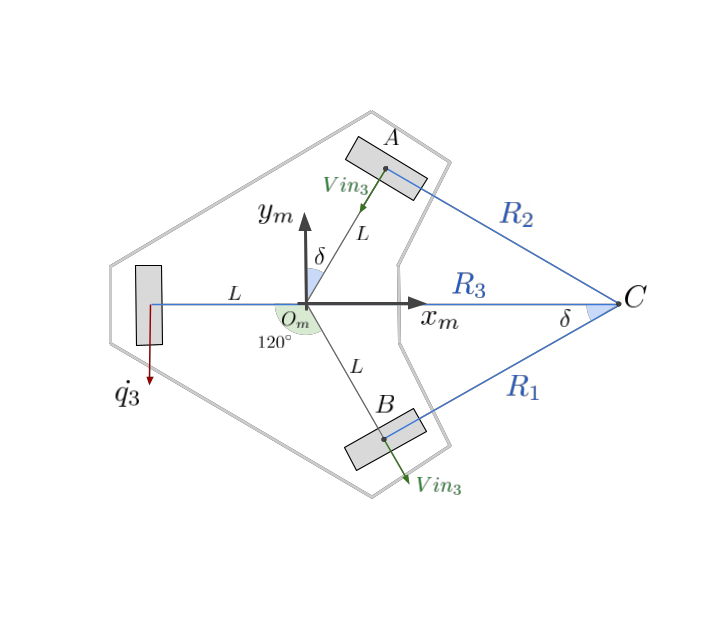
\includegraphics[scale=0.43]{figures/robot3.png}

Looking the triangle $OBC$ we see that:
\begin{equation*}
    \omega = \frac{\dot{q_{3}}}{R_{3}} = \frac{V_{in3}}{R_{1}}         
\end{equation*}

\begin{equation*}
    OC = \sqrt{R_{1}^{2}+L^{2}}= \sqrt{3L^{2}+L^{2}} = 2L
\end{equation*}

\begin{equation*}
    R_{3} = L + OC =3L
\end{equation*}

Since:


\begin{equation*}
    \left\{
        \begin{array}{ll}
            L= OC\sin(\delta) \\
            R_{1}= OC\sin(\frac{\pi}{2} - \delta)
        \end{array}
    \right. \to \left\{
    \begin{array}{ll}
            R_{1}= \frac{\sin(\frac{\pi}{2} - \delta)}{\sin(\delta)}L
            \end{array}
            \right.
\end{equation*}




So:
\begin{equation*}
    R_{1} = \frac{\cos(\delta)}{\sin(\delta)}L
\end{equation*}

\begin{equation*}
    \frac{R_{1}}{R_{3}} = \frac{1}{3}\frac{\cos(\delta)}{\sin(\delta)} \to Vin_{j}= \frac{1}{3}\frac{\cos(\delta)}{\sin(\delta)} \dot{q_{j}}
\end{equation*}


\subsection{General case}
Now, in the general case we have all the three wheels rotating with a specific velocity $\dot{q_{1}}$, $\dot{q_{2}}$, $\dot{q_{3}}$. We can define a local frame $(o,x_{1},y_{1})$ associated with the center of mass of the robot. To obtain the model $RF_{m}$ (The model w.r.t. the robot frame) we have:


\begin{gather}
    ^1V_1 =
    \begin{pmatrix} 
        Vin_3-Vin_2 \\
        \dot{q_{1}}
    \end{pmatrix}
    \\
    ^2V_2 =
    \begin{pmatrix} 
        Vin_1-Vin_3 \\
        \dot{q_{2}}
    \end{pmatrix}
    \\
    ^3V_3 =
    \begin{pmatrix} 
        Vin_2-Vin_1 \\
        \dot{q_{3}}
    \end{pmatrix}
\end{gather}





Considering:
\begin{equation*}
    \left\{
        \begin{array}{ll}
            ^mV_1 = ^mR_1 \quad ^1V_1 \\
            ^mV_2 = ^mR_2 \quad ^2V_2 \\
            ^mV_3 = ^mR_3 \quad ^3V_3
        \end{array}
    \right.
\end{equation*}
And with:
\begin{equation*}
    \left\{
        \begin{array}{ll}
            ^mR_1 = R_{z}(-\frac{\pi}{2}+\delta) \\
            ^mR_2 = R_{z}(\frac{\pi}{2}-\delta) \\
            ^mR_3 = R_{z}(\pi)
        \end{array}
    \right.
\end{equation*}



Where: 
\begin{equation*}
    R_{z}(\alpha) = \begin{pmatrix}
                \cos(\alpha) & -\sin(\alpha)\\
                \sin(\alpha) & \cos(\alpha)
            \end{pmatrix}
\end{equation*}
    
\subsubsection{Model in the robot coordinate system}

We can derive the model w.r.t. the $RF_{m}$:
\begin{equation}
    \left\{
        \begin{array}{ll}
            \begin{pmatrix} 
                \dot{^m x_o} \\ 
                ^m y_o  
            \end{pmatrix} 
            = \frac
                {^m V_1 + ^m V_2 + ^m V_3}
                {3}\\
            
            \omega = \frac{\dot{q_{1}}}{3L} + \frac{\dot{q_{2}}}{3L} + \frac{\dot{q_{3}}}{3L}
        \end{array}
    \right.
\end{equation}
\subsubsection{Model in the world coordinate system}

